\documentclass[crop,tikz]{standalone}% 'crop' is the default for v1.0, before it was 'preview'
%\usetikzlibrary{...}% tikz package already loaded by 'tikz' option
\usepackage{pgfplots}
\pgfplotsset{width=10cm,compat=1.18,ytick style={draw=none},xtick style={draw=none}}

\begin{document}
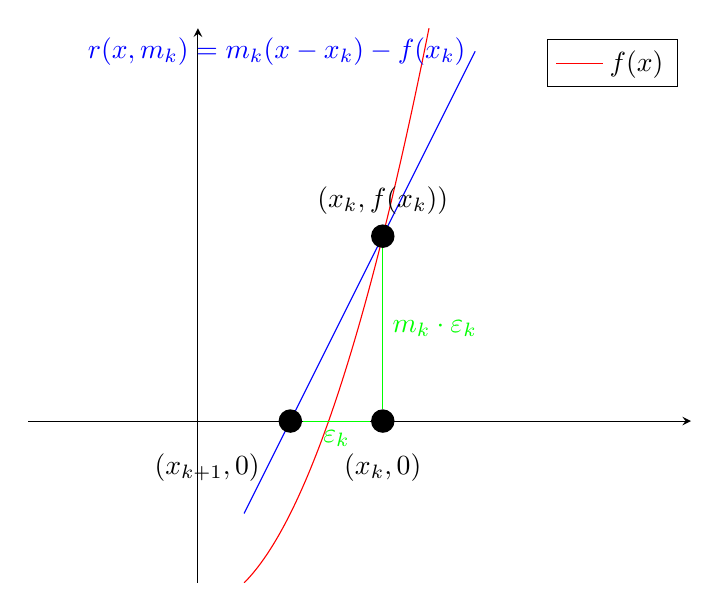
\begin{tikzpicture}
%%%
\begin{axis}[
    axis lines = left,
    %xlabel = \(x\),
    %ylabel = {\(f(x)\)},
    %grid=major, % Display a grid
    grid style={dashed,gray!30},
    axis equal,
    axis x line*=middle,
    axis y line*=middle,
    xtick=\empty,
    ytick=\empty,
]
% f(x)
\addplot [
    domain=0.5:2.5, 
    samples=100, 
    color=red,
]
{x^2 - 2};
\addlegendentry{\(f(x)\)}

% r(m_k, x)
\addplot [
    domain=0.5:3, 
    samples=10, 
    color=blue,
    ]
    {2*x-2} node[left] {\(r(x, m_k) = m_k (x - x_k) - f(x_k) \)};
%\addlegendentry{\(r(x, m_k) = m_k (x - x_k) - f(x_k) \)}

% x, f(x)
\node[label={$\left( x_k, f(x_k)\right)$},circle,fill,inner sep=3pt] at (axis cs:2,2) (C) {};

\node[circle,fill,inner sep=3pt] at (axis cs:1,0) (A) {};
\node at (axis cs:0.1,-0.5) {$\left(x_{k+1},0\right)$};

\node[circle,fill,inner sep=3pt] at (axis cs:2,0) (B) {};
\node at (axis cs:2,-0.5) {$\left(x_{k},0\right)$};

\draw[color=green] (A) -- (B) node[midway,below] {$\varepsilon_k$};
\draw[color=green] (B) -- (C) node [midway, right] {$m_k \cdot \varepsilon_k$};

\end{axis}
%%%
\end{tikzpicture}
\end{document}